\section{Προθεματικοί Αθροιστές}
Στην ενότητα αυτή θα παρουσιαστεί μια νέα προσέγγιση των αθροιστών, οι αθροιστές προθέματος, οι οποίοι έλαβαν σημαντικό ρόλο στην επιτάχυνση παραλληλοποιώντας την διαδικασία υπολογισμού των κρατουμένων στους αθροιστές πρόβλεψης κρατουμένου που περιγράφηκαν στο προηγούμενο κεφάλαιο. Οι αθροιστές προθέματος που ακολουθούν αποτελούν τροποποίηση της μονάδας υπολογισμού των κρατουμένων.





\subsection{Πρόβλημα προθέματος}

Ένα πρόβλημα προθέματος ή prefix problem
ορίζεται από n εξόδους y ( $y_{n-1},y_{n-2}, ... ,y_0 $ ) , n εισόδους x ( $x_{n-1},x_{n-1}, ... ,x_0 $ ) και τον τελεστή $\circledast$ .
Κάθε έξοδος y υπολογίζεται με τον παρακάτω τρόπο :
\begin{equation}
\begin{split}
y_0 &= x_0\\
y_1 &= x_1 \circledast x_0\\
y_2 &= x_2 \circledast x_1 \circledast x_0\\
&...\\
y_{n-1} &= x_{n-1} \circledast x_{n-2} \circledast ... \circledast x_{1} \circledast x_0\\
\end{split}
\end{equation}

Είναι επίσης δυνατή και η αναδρομική έκφραση :
\begin{equation}
\begin{split}
y_0 &= x_0\\
y_{i} &= x_{i} \circledast y_{i-1}\\
\end{split}
\end{equation}

Ένα απλό παράδειγμα προβλημάτων που αντιμετωπίζονται ως προβλήματα προθέματος είναι 
η πρόσθεση πολλών αριθμών. Έστω ένα σύνολο μεγέθους n από αριθμούς 
$(x_{n-1},x_{n-2}, ... ,x_1,x_0)$, σύμφωνα με τον ορισμό που δόθηκε παραπάνω
ορίζεται ένα ακόμα σύνολο ίδιου μεγέθους $(y_{n-1},y_{n-2}, ... ,y_1,y_0)$ 
όπου κάθε στοιχείο του συνόλου αυτού υπολογίζεται αναδρομικά, σύμφωνα με την παρακάτω εξίσωση
\begin{equation*}
\begin{split}
y_0 &= x_0\\
y_{i} &= x_{i} + y_{i-1}\\
\end{split}
\end{equation*}
και το τελικό αποτέλεσμα καταχωρείται στο $y_{n-1}$.

Το πρόβλημα υπολογισμού κρατουμένου είναι δυνατόν να μετατραπεί σε
προθεματικό πρόβλημα δημιουργώντας τα ζεύγη $(G,P)$ και αναθέτοντας στον τελεστή
$\circledast$ την παρακάτω λειτουργιά :
\begin{equation}
\begin{split}
(g_i,p_i) \circledast (g_k,p_k) &= (g_i + p_ig_k , p_ip_k)\\
(G_i,P_i) \circledast (G_k,P_k) &= (G_i + P_iG_k , P_iP_k)
\end{split}
\end{equation}

Με αυτόν τον τρόπο υπολογίζεται κάθε ενδιάμεσο κρατούμενο $c_i$
καθώς και το κρατούμενο εξόδου $c_n$ για έναν αθροιστή των n-bits όπου $c_i = G_i$
και για $n \geq i \geq 0$ έχουμε 
\begin{equation}
\equationame{Αλγεβρικός ορισμός των $(G_i,P_i)$}
\begin{split}
(G_0,P_0) &= (g_0,p_0)\\
(G_i,P_i) &= (g_i,p_i) \circledast (G_{i-1},P_{i-1})
\end{split}
\end{equation}
Παρακάτω ακολουθεί η επαγωγική απόδειξη.
Εφόσον δεν υπάρχει κρατούμενο εισόδου ($c_{in} = c_{-1} = 0$) έχουμε 
\begin{equation*}
\begin{split}
    c_0 &= g_0 + p_0c_{-1} \\
    c_0 &= g_0 \\
    c_0 &= G_0
\end{split}
\end{equation*}
έστι το αποτέλεσμα ισχύει για $i-1$ \\
Αν $i>0$ και $c_{i-1} = G_{i-1}$ τοτε
\begin{equation*}
\begin{split} 
    (G_i,P_i)   &= (g_i,p_i) \circledast (G_{i-1},P_{i-1}) \\
                &= (g_i,p_i) \circledast (c_{i-1},P_{i-1}) \\
                &= (g_i + p_ic_{i-1} , p_iP_{i-1}) \\
            G_i &= g_i + p_ic_{i-1} \\
            G_i &= c_i
\end{split}
\end{equation*}
Επίσης, ο τελεστής $\circledast$ έχει προσεταιριστική ιδιότητα 
\begin{equation*}
\begin{split} 
    (g_i,p_i)\circledast(g_j,p_j)\circledast(g_k,p_k) &= [g_i + p_ig_j,p_ip_j]\circledast(g_k,p_k) \\
    &= (g_i,p_i)\circledast[g_j + p_jg_k,p_jp_k]\\
    &= ( g_i + p_ig_j + p_ip_jg_k , p_ip_jp_k )
\end{split}
\end{equation*}

Στην εικόνα \ref{Serial-PrefixTree} παρουσιάζεται ένα γράφημα-δέντρο ενός απλού αθροιστή διάδοσης κρατουμένου, αναγόμενο σε πρόβλημα προθέματος.\\ 
\begin{figure}[H]
\centering
% 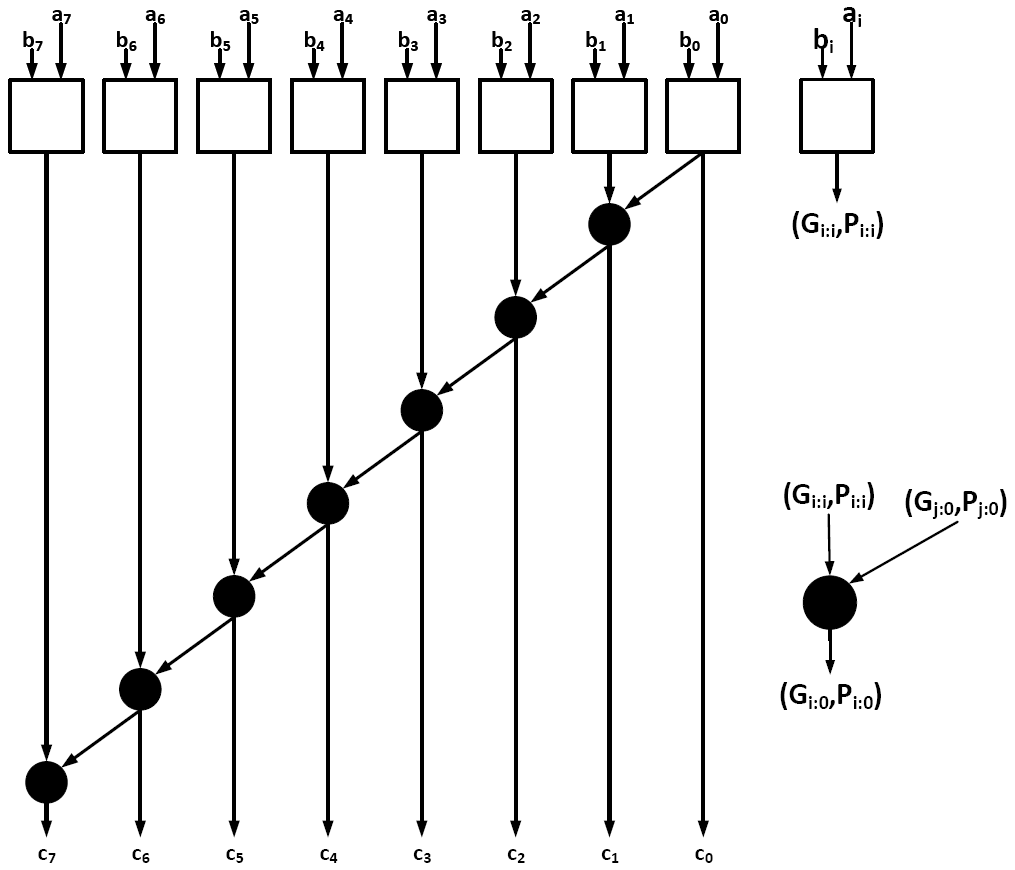
\includegraphics[width=\textwidth]{Serial-Prefix.png}
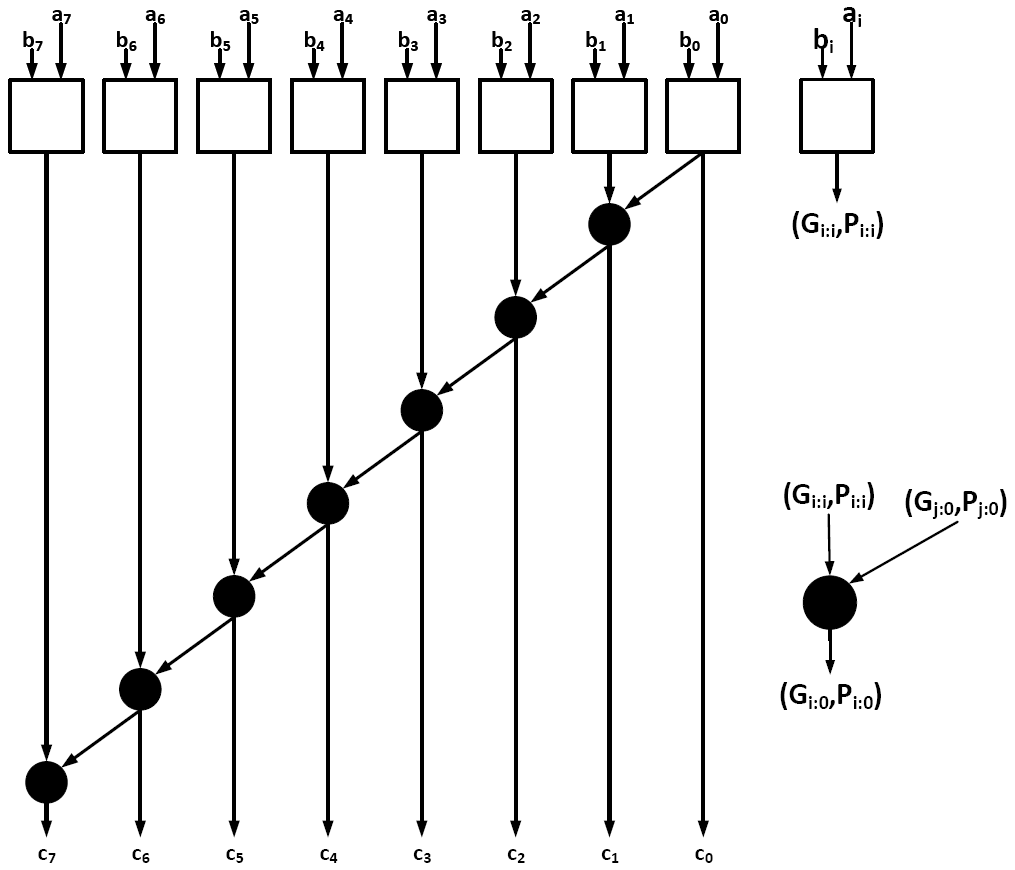
\includegraphics[scale=0.4]{Serial-Prefix.png}
\caption{Σειριακή προθεματική δομή του αθροιστή}
\label{Serial-PrefixTree}
\end{figure}
Σε κάθε μαύρο κόμβο ουσιαστικά υλοποιείται η λογική συνάρτηση του τελεστή $\circledast$
που παρουσιάστηκε προηγουμένως. Ο παραπάνω αθροιστής υλοποιεί τον προθεματικό αλγόριθμο
σειριακά με αποτέλεσμα να είναι πολύ αργό το μοντέλο αλλά να καταλαμβάνει μικρότερο εμβαδόν
σε σχέση με άλλες τοπολογίες αθροιστών προθέματος που θα παρουσιαστούν στην συνέχεια. Σημειώνεται πως λιγότεροι κόμβοι συνεπάγεται μικρότερο εμβαδόν.












\subsection{Παράλληλοι Προθεματικοί Αθροιστές}
Η διάταξη που παρουσιάστηκε στην εικόνα \ref{Serial-PrefixTree} έχει την δομή 
του απλού αθροιστή διάδοσης κρατουμένου εκφρασμένο σε προθεματική μορφή. Ο προθεματικός
όμως υπολογισμός κρατουμένων μπορεί να υπολογιστεί παράλληλα, αποτελώντας την προθεματική 
έκφραση ως κινητήριο παράγοντα διάφορων παράλληλων αρχιτεκτονικών που προτάθηκαν.
Μερικές σημαντικές αρχιτεκτονικές διατυπώνονται στις επόμενες παραγράφους με σύντομη
περιγραφή.




\subsubsection{Δέντρα-Δομές Προθεμάτων}


\subsubsection*{J. Sklansky}
Μία από τις πρώτες παράλληλες τοπολογίες που προτάθηκε ήταν το 1960 απο τον Sklansky \cite{5219822}. Το πλεονέκτημα της είναι το ελάχιστο βάθος. Στην εικόνα \ref{SklanskyTree} παρουσιάζεται ένα παράδειγμα υπολογισμού των κρατουμένων για είσοδο των οκτώ δυαδικών ψηφίων. Το βάθος σε αυτή την περίπτωση είναι τρία επίπεδα. Παρατηρείται πως ο κόμβος του κρατουμένου $c_3$ εκτός από το ίδιο το κρατούμενο οδηγεί επιπλέον τέσσερις εισόδους αλλών κόμβων (Fan-out -4). Το υψηλό Fan-Out των κόμβων είναι το σημείο στο οποίο μειονεκτεί ο σχεδιασμός αυτός.
\begin{figure}[H]
    \centering
    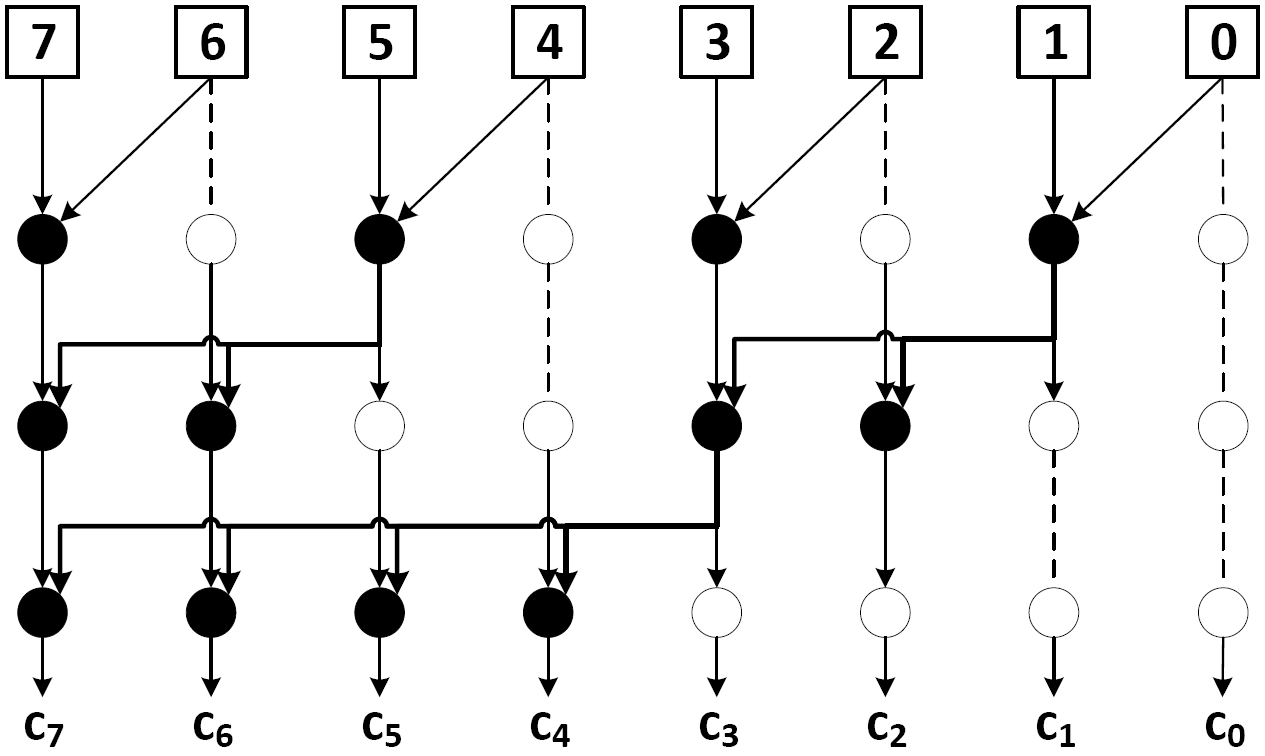
\includegraphics[scale=0.27]{Sklansky.png}
    \caption{J. Sklansky Προθεματικό Δέντρο αθροιστή}
    \label{SklanskyTree}
\end{figure}
Το 1980 παρουσιάστηκε μια αρχιτεκτονική από τους Ladner και Fischer 
\cite{Ladner:1980:PPC:322217.322232} η οποία είχε την ίδια βασική δομή με αυτή του
Sklansky, με κάποιες τροποποιήσεις ανάλογα την εφαρμογή, για καλύτερη απόδοση.




\clearpage
\subsubsection*{Kogge-Stone}
Όπως και η αρχιτεκτονική που προτάθηκε από τον Sklansky, έτσι και η αρχιτεκτονική
Kogge-Stone \cite{5009159} έχει μικρό βάθος. Η βασική του όμως διαφορά είναι πως δεν υπάρχει 
κόμβος με μεγαλύτερο του δυο fan-out, θυσιάζοντας το εμβαδόν του σχεδιασμού.
\begin{figure}[H]
    \centering
    %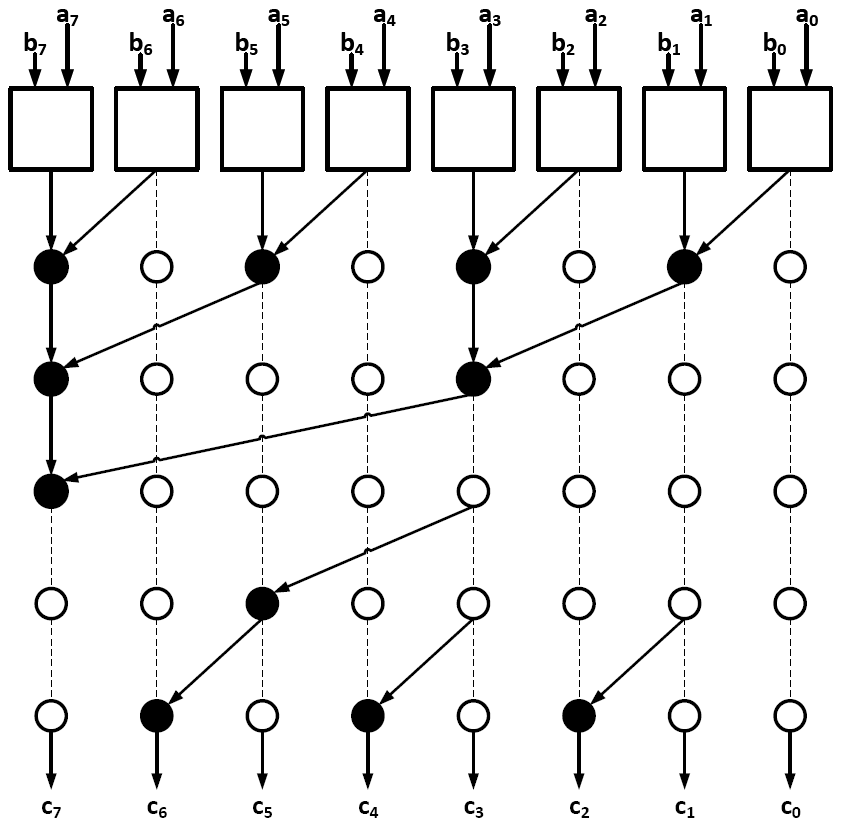
\includegraphics[width=\textwidth]{Brent_Kung_Prefix.png}
    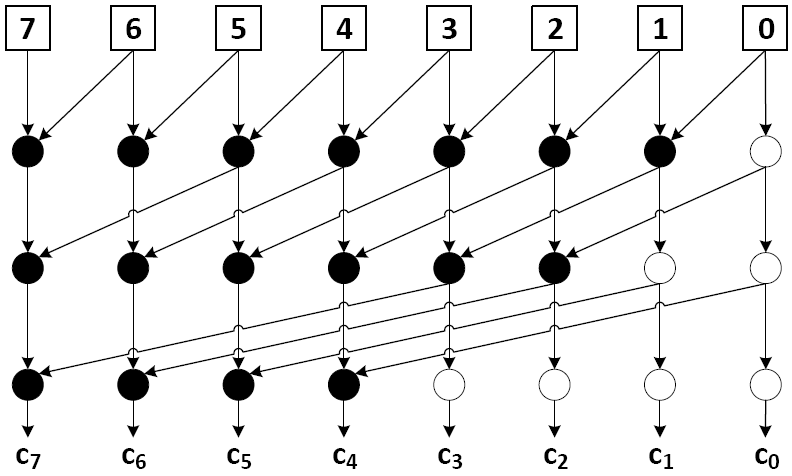
\includegraphics[scale=0.45]{Pictures/Kogge-Stone.png}
    \caption{Kogge-Stone Προθεματικό Δέντρο αθροιστή}
    \label{Kogge-StoneTree}
\end{figure}






\subsubsection*{Brent-Kung}
Στην περίπτωση της δομής Brent-Kung \cite{Brent:1982:RLP:1309296.1309891}
όπως φαίνεται και στην εικόνα \ref{BrentKungTree} παρουσιάζει μεγάλο βάθος αλλά καταλαμβάνει
λιγότερο εμβαδόν.
\begin{figure}[H]
    \centering
    %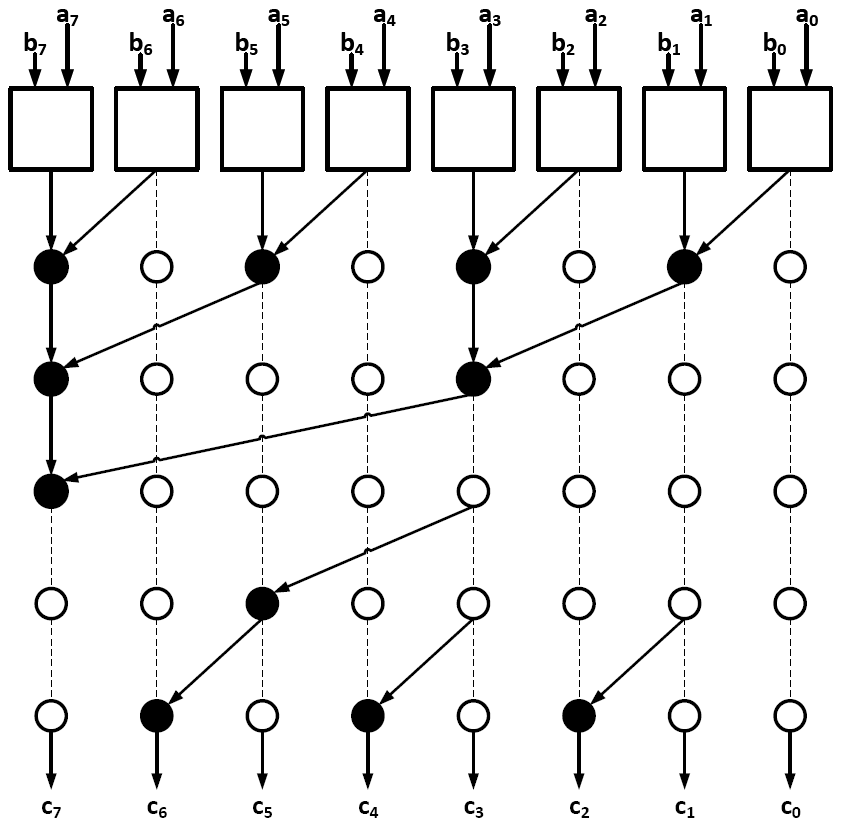
\includegraphics[width=\textwidth]{Brent_Kung_Prefix.png}
    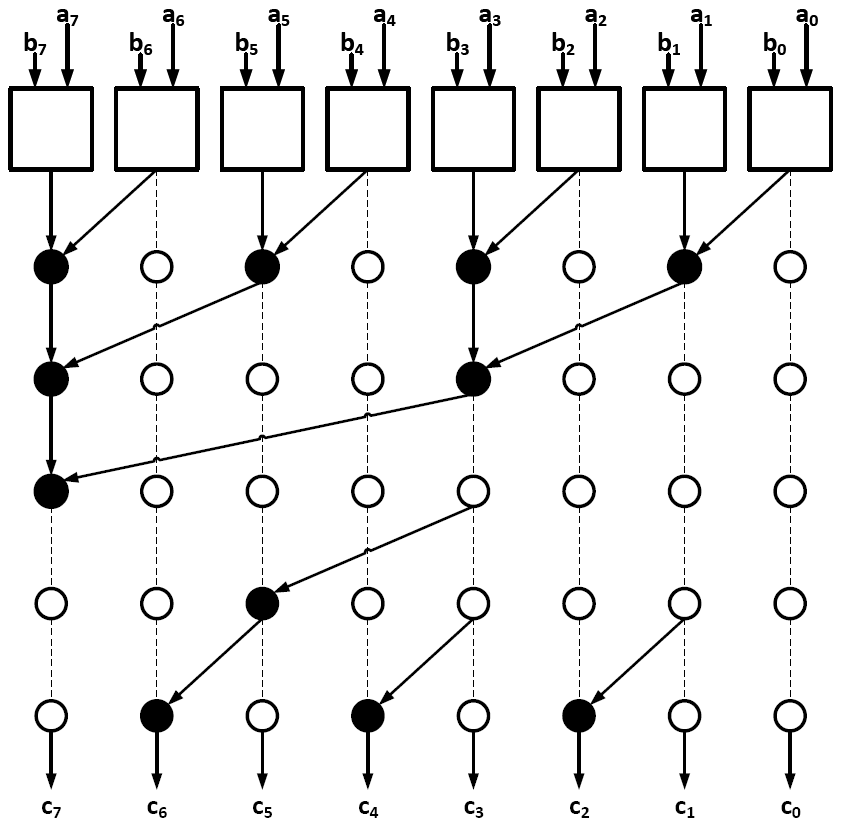
\includegraphics[height=6cm,width=9cm]{Brent_Kung_Prefix.png}
    \caption{Brent-Kung Προθεματικό Δέντρο αθροιστή}
    \label{BrentKungTree}
\end{figure}




\subsubsection*{Σύγκριση των παράλληλων διατάξεων}

Στον πίνακα \ref{Prefix_Comparison} εκφράζεται μαθηματικα το πλήθος των επιπέδων, το πλήθος των 
κόμβων και το μέγιστο Fan-Out ανα αθροιστή, ανάλογα με το μήκος εισόδου του $n$.
\begin{table}[H]
\centering
     \begin{tabular}{  c c c c  } 

        \hline
        Architecture & Levels(Delay) & nodes(Area) & max fan-out\\
        \hline
        
        Serial &
        $n-1$ &
        $n-1$ &
        $2$\\
        
        Sklansky &
        $\log_2 n$ &
        $n/2\log_2n$ &
        $n/2+1$\\
        
        Kogge-Stone &
        $\log_2n$ &
        $n(\log_2n-1)+1$ &
        $2$\\
        
        Brent-Kung &
        $2\log_2n-1$ &
        $ 2(n-1) - \log_2n $ &
        $\log_2n+1$\\
        
        \hline

    \end{tabular}

\caption{Σύγκριση των Προθεματικών Δέντρων}
\label{Prefix_Comparison}
\end{table}
Στις προθεματικές τοπολογίες που παρουσιάζονται σε αυτή την εργασία κάθε επίπεδο θεωρητικά έχει 
την ίδια χρονική καθυστέρηση με τα υπόλοιπα επίπεδα. Η παραδοχή αυτή στηρίζεται στο ότι 
σε κάθε επίπεδο, κάθε κόμβος είναι παράλληλα ή ανεξάρτητος συνδεδεμένος με τους υπόλοιπους
του ίδιου επιπέδου, με αποτέλεσμα το κρίσιμο μονοπάτι του επιπέδου να είναι ίσο με αυτό του
κόμβου. Συμπεραίνετε λοιπόν πως κάθε επίπεδο έχει ίδια καθυστέρηση και ίση με την καθυστέρηση
ενός κόμβου. Αποτέλεσμα του ισχυρισμού αυτού είναι η συσχέτιση του πλήθους των επιπέδων με 
την συνολική καθυστέρηση του αθροιστή.

Η παραπάνω αναλογία μεταξύ των επιπέδων και της καθυστέρησης έχει εφαρμογή και σε φυσικές
υλοποιήσεις των προθεματικών αθροιστών. Συγκρίνοντας τους αθροιστές Kogge-Stone και Sklansky ως
προς την ταχύτητα, σύμφωνα με τον παραπάνω ισχυρισμό θα ήταν αναμενόμενο να έχουν την ίδια 
απόδοση. Συμπεριλαμβάνοντας και το εμβαδόν στην εξίσωση επιλογής ταχύτερου αθροιστή, ως δευτερεύον
παράγοντα, το πρόβλημα τείνει στην επιλογή του Sklansky. Ο λόγος όμως που η αρχιτεκτονική 
Kogge-Stone είναι ιδανική αφορά το μικρό fan-out. Στην περίπτωση κυκλώματος με κόμβους
που έχουν υψηλό fan-out, είναι αναγκαία η πρόσθεση ηλεκτρονικών στοιχείων για την σωστή οδήγηση
με αποτέλεσμα να επιβαρύνετε το σύστημα χρονικά.














\subsection{Αραίωση των Δέντρων}
\label{subsection:prefix_sparseness}
Οι δομές που περιγράφηκαν για την παραλληλοποίηση του υπολογισμού των κρατουμένων 
είναι αρκετά πυκνές όσον αφορά τους κόμβους, το οποίο συνεπάγει υψηλές απαιτήσεις πόρων υλικού και ενέργειας. Με σκοπό την μείωση του εμβαδού εφαρμόζονται τεχνικές αραίωσης ή sparseness. Οι τεχνικές αυτές βασίζονται στον υπολογισμό λιγότερων κρατούμενων από των απαιτούμενων και την διάδοση αυτών για τον υπολογισμό των υπόλοιπων. Μειονέκτημα αυτής της τεχνικής είναι η αύξηση της λογικής πολυπλοκότητας του τελευταίου επιπέδου όπου πραγματοποιείται η άθροιση, με αποτέλεσμα την μείωση της ολικής χρονικής απόδοσης.

\begin{figure}[H]
    \centering
    %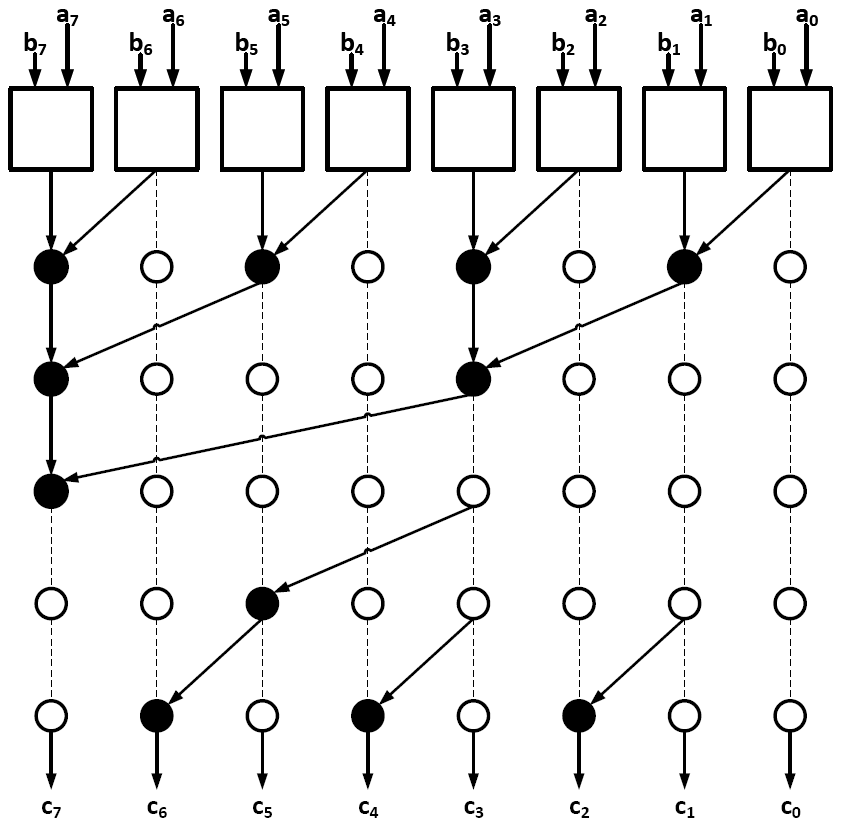
\includegraphics[width=\textwidth]{Brent_Kung_Prefix.png}
    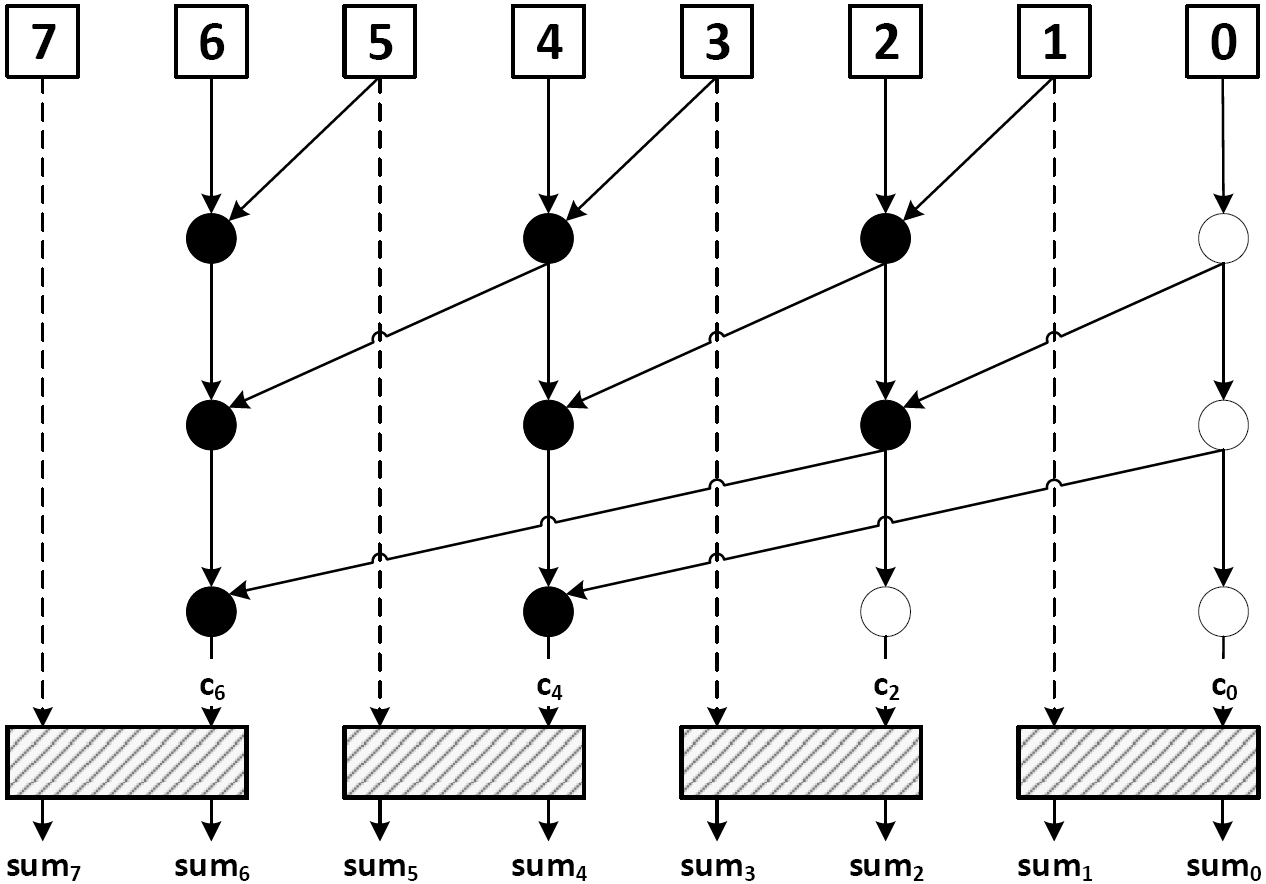
\includegraphics[height=7cm,width=9cm]{Pictures/prefix_sparse_2.png}
    \caption{Προθεματικός αθροιστής με τεχνική αραίωσης}
    \label{fig:prefix_sparse_2}
\end{figure}

Στην εικόνα \ref{fig:prefix_sparse_2} παρουσιάζεται το διάγραμμα ενός αθροιστή οκτώ δυαδικών ψηφίων με την εφαρμογή της τεχνικής αραίωσης sparse-2, δηλαδή υπολογίζονται τα μισά κρατούμενα (ανά δύο), στην δομή Kogge-Stone. Στις εξισώσεις που ακολουθούν περιγράφεται η διάδοση των κρατουμένων στο τελευταίο επίπεδο για τεχνική αραίωσης sparse-2 και sparse-4.\\\\
Sparsness-2
\begin{equation*}
    \begin{split}
        sum_i &= x_i \oplus G_{i-1:0}\\
        sum_{i+1} &= x_{i+1} \oplus G_{i:0}\\
        &= x_{i+1} \oplus (g_i + p_i*G_{i-1:0})\\
    \end{split} 
\end{equation*}
Sparsness-4
\begin{equation*}
    \begin{split}
        sum_i &= x_i \oplus G_{i-1:0}\\
        sum_{i+1} &= x_{i+1} \oplus G_{i:0}\\
        &= x_{i+1} \oplus (g_i + p_i*G_{i-1:0})\\
        sum_{i+2} &= x_{i+2} \oplus G_{i+1:0}\\
        &= x_{i+2} \oplus (g_{i+1} + p_{i+1}g_i + p_{i+1}p_iG_{i-1:0})\\
        sum_{i+3} &= x_{i+3} \oplus G_{i+2:0}\\
        &= x_{i+3} \oplus (g_{i+2} + p_{i+2}g_{i+1} + p_{i+2}p_{i+1}g_i + p_{i+2}p_{i+1}p_iG_{i-1:0})\\
    \end{split} 
\end{equation*}


















\subsection{Προθεματικός αθροιστής με κρατούμενο εισόδου}
Οι αθροιστές προθέματος που παρουσιάστηκαν παραπάνω αναπτύχθηκαν με την αρχική
υπόθεση έλλειψης κρατουμένου εισόδου ή $c_{in} = 0$. Ενσωματώνοντας στους παραπάνω 
αθροιστές την επιλογή κρατουμένου εισόδου $c_{in}$, το οποίο ταυτίζεται με το σήμα $c_{-1}$
, ορίζεται το αντίστοιχο ζεύγος σημάτων $(G'_i,P'_i)$, όπου είναι το Grou Generate και 
Group Propagate αντίστοιχα με την διαφορά πως συμπεριλαμβάνουν και το κρατούμενο εισόδου.
Ακολουθεί ο αλγεβρικός ορισμός των σημάτων $G'_i$ και $P'_i$ ( εξίσωση \ref{eq:GP_with_carry_in} )
\begin{equation}
    \equationame{Αλγεβρικός ορισμός των $(G'_i,P'_i)$}
    \label{eq:GP_with_carry_in}
    (G'_i,P'_i) = 
    \begin{cases}
        (g_0 + p_0*c_{-1} , p_0)   , & i = 0\\
        (g_i,p_i)\circledast (G'_{i-1},P'_{i-1}) , & 1 \leq i \leq n-1
    \end{cases}
\end{equation}
Επίσης, στην περίπτωση που συνυπολογίζεται και το κρατούμενο εισόδου, προφανώς ισχύει και 
$c_i = G'_i$. Για την ανάκτηση των $(G'_i,P'_i)$ χρησιμοποιείται ο παρακάτω τύπος:
\begin{equation}
    \label{eq:G'P'_From_GP}
    \equationame{Ανάκτηση των $(G'_i,P'_i)$ από $(G_i,P_i)$}
    (G'_i,P'_i) = (G_i + P_i*c_{-1} , P_i)
\end{equation}
το οποίο αποδεικνύεται επίσης επαγωγικά στο $i$. Για $i=0$ ισχύει :
\begin{equation*}
    (G'_0,P'_0) = (g_0 + p_0*c_{-1} , p_0) =  (G_0 + P_0*c_{-1} , P_0)
\end{equation*}
Υποθέτοντας πως η σχέση ισχύει και για $i=k-1$, δηλαδή
\begin{equation*}
    (G'_{k-1},P'_{k-1}) = (G_{k-1} + P_{k-1}*c_{-1} , P_{k-1})
\end{equation*}
Τότε για $i=k$ :
\begin{equation*}
    \begin{split}
        (G'_k,P'_k) &= (g_k,p_k) \circledast (G'_{k-1},P'_{k-1})\\
                    &= (g_k,p_k) \circledast (G_{k-1} + P_{k-1}*c_{-1} , P_{k-1}) \\
                    &= ( g_k + p_k*(G_{k-1} + P_{k-1}*c_{-1}) , p_k*P_{k-1} ) \\
                    &= \big( (g_k + p_kG_{k-1}) + p_kP_{k-1}c_{-1} , P_k  \big) \\
                    &= ( G_k + P_k*c_{-1} , P_k )
    \end{split}
\end{equation*}

Όσον αφορά την τροποποίηση των γραφημάτων για τον συνυπολογισμό κρατουμένου εισόδου
είναι δυνατό να κρατηθεί ανέπαφη η δομή υπολογίζοντας τα Group Generate και Group Propagate 
$(G_i,P_i)$ χωρίς το κρατούμενο εισόδου  και στο τέλος προστίθεται ένα ακόμα επίπεδο
για κάθε δυαδικό ψηφίο $i$ που υλοποιείται η λογική $G_ι + P_ι*c_{-1}$.
Στην εικόνα \ref{Kogge-StoneTree_with_carry_in} παρουσιάζεται ένα παράδειγμα προθεματικού αθροιστή
με κρατούμενο εισόδου. Εντός του σκιασμένου πλαισίου είναι δυνατό να εφαρμοστεί οποιαδήποτε 
προθεματική δομή (χωρίς κρατούμενο εισόδου). Στο παράδειγμα αυτό χρησιμοποιήθηκε η 
αρχιτεκτονική του Kogge-Stone.
\begin{figure}[H]
    \centering
    %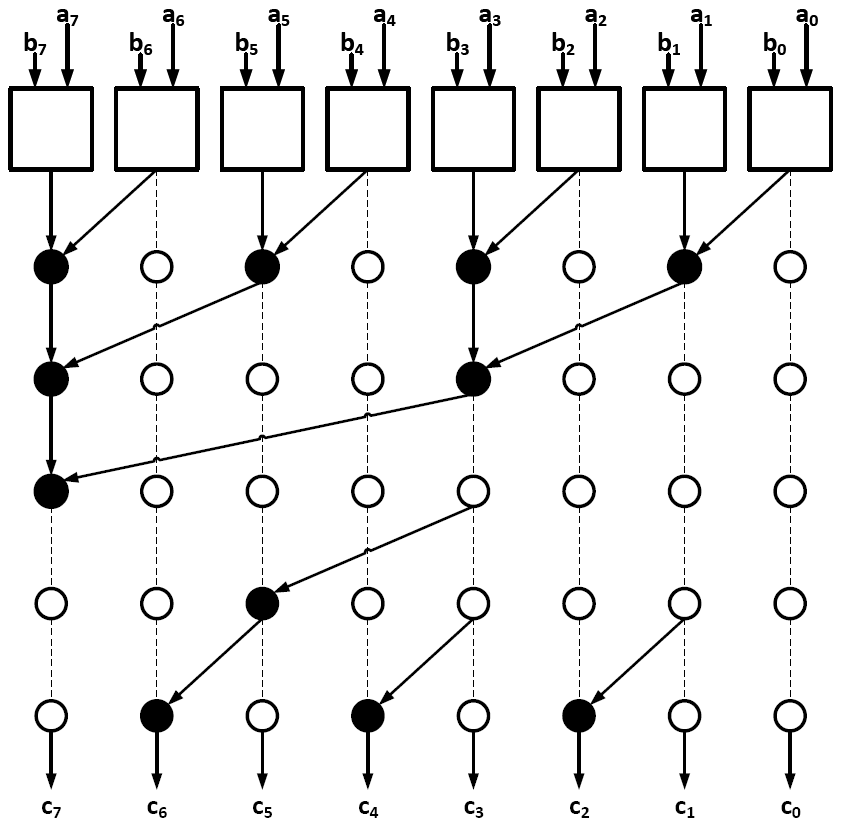
\includegraphics[width=\textwidth]{Brent_Kung_Prefix.png}
    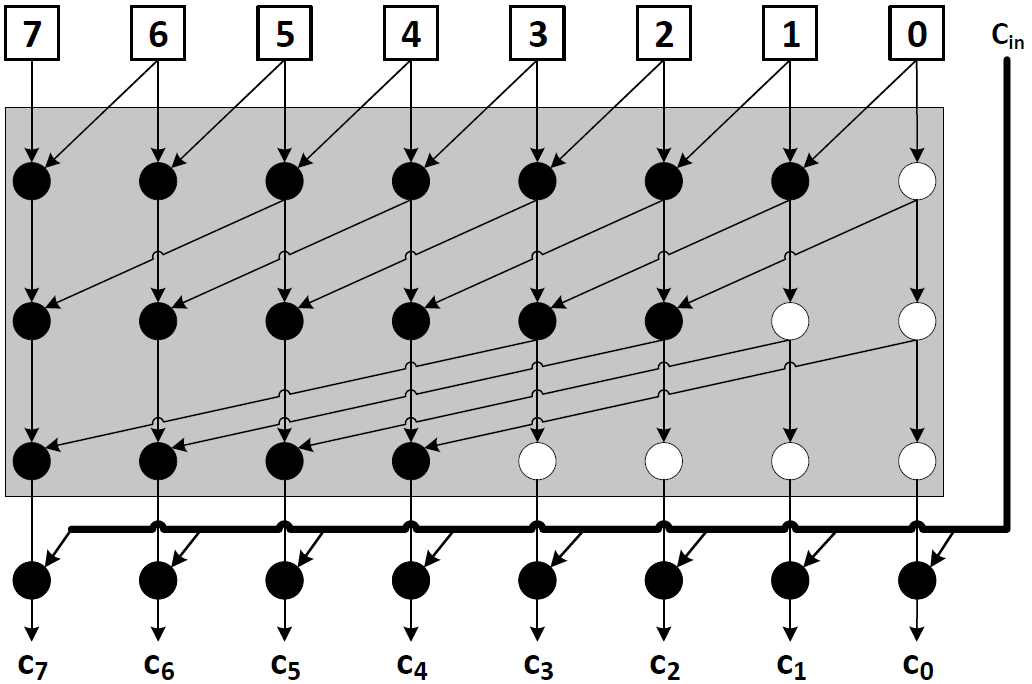
\includegraphics[height=7cm,width=10cm]{Pictures/Kogge-stone_with_carry_in.png}
    \caption{Kogge-Stone Δέντρο Προθεματικού αθροιστή με κρατούμενο εισόδου}
    \label{Kogge-StoneTree_with_carry_in}
\end{figure}

